%% IEEEtran — conference paper
\documentclass[conference]{IEEEtran}

\usepackage[utf8]{inputenc}
\usepackage[T1]{fontenc}
\usepackage{amsmath,amssymb}
\usepackage{graphicx}
\usepackage{booktabs}
\usepackage{xcolor}
\usepackage{hyperref}
\usepackage{cite}
\usepackage{url}

\hypersetup{
  colorlinks=true,
  linkcolor=blue,
  citecolor=blue,
  urlcolor=blue
}

% Marca visual para resultados pendientes de correr con el dataset real
\newcommand{\pending}[1]{\textcolor{red}{[PENDIENTE: #1]}}

\begin{document}

\title{Detecting AI-Generated Veterinary Radiographs:\\
A Dual-Stream Approach Against Pet Insurance Fraud}

\author{
  \IEEEauthorblockN{Juan Manuel Castillo Pinto}
  \IEEEauthorblockA{
    Maestría en Inteligencia Artificial\\
    Universidad de La Salle, Bogotá, Colombia\\
    jmmana@gmail.com
  }
}

\maketitle

% -------------------------------------------------------
\begin{abstract}
Generative models can now synthesize medical images realistic enough to deceive both human experts and automated systems, a risk recently confirmed for human radiographs by a 2026 RSNA study in which board-certified radiologists misclassified roughly one in five AI-generated chest X-rays as authentic. This vulnerability directly threatens insurance underwriting, where fraudulent diagnostic imagery can be used to inflate or fabricate claims. While medical deepfake detection has received growing attention in human radiology (e.g., MedForensics, M3Dsynth), no prior published dataset or method addresses \emph{veterinary} diagnostic imaging, despite documented and costly fraud in the pet insurance industry, estimated at 3--7 loss-ratio points (USD 300K--700K per USD 10M in premium). This paper introduces (1) a legally re-distributable dataset of canine thoracic radiographs paired with AI-generated synthetic counterparts, built by re-licensing an existing CC BY 4.0 Mendeley Data collection and augmenting it with a trained generative adversarial network, and (2) a dual-stream detector combining spatial CNN features (ResNet-18) with a radially-averaged frequency-domain descriptor designed to expose the periodic upsampling artifacts characteristic of GAN-based generation. We release the resulting dataset publicly on Kaggle to seed further research in this unexplored niche. \pending{completar con metricas finales: accuracy, AUC, precision, recall sobre el conjunto de prueba}.
\end{abstract}

\begin{IEEEkeywords}
veterinary radiology, medical deepfake detection, generative adversarial networks, insurance fraud, frequency-domain forensics, synthetic medical imaging
\end{IEEEkeywords}

% -------------------------------------------------------
\section*{Resumen (Spanish Abstract)}
Los modelos generativos ya pueden sintetizar imagenes medicas suficientemente realistas como para enganar tanto a expertos humanos como a sistemas automaticos, un riesgo confirmado en 2026 por un estudio de la RSNA en el que radiologos certificados clasificaron erroneamente como autenticas cerca de una de cada cinco radiografias de torax generadas por IA. Esta vulnerabilidad amenaza directamente la suscripcion de polizas de seguros, donde una imagen diagnostica fraudulenta puede usarse para inflar o fabricar un reclamo. Mientras la deteccion de deepfakes medicos ha recibido atencion creciente en radiologia humana (MedForensics, M3Dsynth), ningun dataset ni metodo publicado aborda la imagen diagnostica \emph{veterinaria}, pese a que el fraude en seguros de mascotas es un problema documentado y costoso para la industria (entre 3 y 7 puntos de loss ratio, 300 mil a 700 mil dolares por cada 10 millones en primas). Este articulo presenta un dataset legalmente redistribuible de radiografias caninas de torax junto con contrapartes sinteticas generadas por IA, construido re-licenciando una coleccion CC BY 4.0 de Mendeley Data y aumentandola con una red generativa adversarial entrenada, y un detector de dos ramas que combina caracteristicas espaciales (ResNet-18) con un descriptor de frecuencia que expone los artefactos periodicos del proceso de upsampling. El dataset resultante se publica en Kaggle para sembrar investigacion futura en este nicho inexplorado.

% -------------------------------------------------------
\section{Introduction}
\label{sec:intro}

Generative adversarial networks (GANs) and diffusion models have reached a level of visual fidelity that makes synthetic medical images increasingly difficult to distinguish from real acquisitions. A controlled study published through RSNA in March 2026 exposed board-certified radiologists and multimodal large language models to a mixed set of 264 authentic and AI-generated chest radiographs (produced with tools including ChatGPT-based generators and Stanford's RoentGen model); accuracy ranged from 58\% to 92\% among human readers, meaning a meaningful fraction of fabricated images escaped detection entirely \cite{rsna_deepfake_xray_2026}. The same report explicitly names insurance fraud, litigation, and factitious disorder (Munchausen syndrome) as realistic misuse scenarios \cite{rsna_deepfake_xray_2026}.

This risk is not hypothetical for the pet insurance industry. Unlike human healthcare systems, veterinary medical records do not travel between clinics: there is no shared infrastructure to verify an animal's diagnostic history across providers. Industry analyses estimate that claims fraud costs pet insurance managing general agents (MGAs) 3--7 points of loss ratio, translating to USD 300K--700K per USD 10M in written premium, while noting that even basic rules-based detection programs deliver a 3--10x return on investment \cite{insurnest_fraud_2026}. As image-editing and generative tools become trivially accessible, fabricated or altered diagnostic imagery (a forged fracture, an exaggerated lesion) is a natural next step for claims fraud, exactly mirroring the human-healthcare threat already demonstrated at RSNA.

Despite this, a review of the medical deepfake detection literature reveals that every existing dataset and method targets \emph{human} imaging modalities. MedForensics, presented at MICCAI 2025, spans six human modalities (ultrasound, endoscopy, histopathology, MRI, CT, X-ray) and twelve generative models, explicitly measuring cross-generator generalization \cite{medforensics2025}. M3Dsynth addresses AI-generated local manipulations in human 3D medical volumes \cite{m3dsynth2023}. A 2026 study directly comparing GAN- and diffusion-generated fakes reports the same generalization gap using human skin-cancer imagery \cite{hybrid_gan_diffusion_2026}. None of this work, nor any dataset we could locate on Kaggle or elsewhere, considers veterinary diagnostic images.

This paper makes three contributions:
\begin{enumerate}
  \item A legally clear, publicly re-distributed dataset of canine thoracic radiographs paired with GAN-generated synthetic counterparts, built by re-licensing an existing CC BY 4.0 dataset and republishing it on Kaggle with correct attribution to the original authors.
  \item A dual-stream detector architecture that fuses spatial CNN features with a frequency-domain descriptor, adapted from the human-imaging forensics literature to a new, data-scarce veterinary domain.
  \item An honest characterization of what a small, real, publicly available veterinary imaging dataset can and cannot support, intended as a reproducible starting point rather than a production-ready fraud detection system.
\end{enumerate}

The remainder of this paper is organized as follows. Section~\ref{sec:related} reviews related work on medical deepfake generation and detection. Section~\ref{sec:dataset} describes the dataset and its licensing chain. Section~\ref{sec:method} presents the generation and detection methodology. Section~\ref{sec:experiments} describes the experimental setup. Section~\ref{sec:results} reports results. Section~\ref{sec:discussion} discusses limitations and future work, and Section~\ref{sec:conclusion} concludes.

% -------------------------------------------------------
\section{Related Work}
\label{sec:related}

\subsection{Synthetic medical image generation}
GANs and diffusion models are both used to synthesize medical images across modalities including MRI, CT, X-ray, ultrasound, and dermoscopy, motivated primarily by data augmentation and privacy-preserving data sharing \cite{synthetic_review_2026}. Diffusion models have recently overtaken GANs in perceptual image quality, including for chest X-ray generation, but their clinical reliability and the artifacts they leave behind remain comparatively underexplored relative to GANs \cite{synthetic_review_2026}.

\subsection{Detecting AI-generated medical images}
MedForensics is, to our knowledge, the most comprehensive published benchmark for medical deepfake detection, spanning six modalities and twelve generative models, and proposes DSKI, a dual-stage knowledge-infusing detector built on a vision-language feature space that outperforms prior methods and human experts in a visual Turing test \cite{medforensics2025}. Its architecture uses three parallel CNN streams targeting visual perception, resampling artifacts, and local inconsistency. M3Dsynth focuses on localized manipulations within 3D volumes rather than whole-image synthesis \cite{m3dsynth2023}. A 2026 study on skin-cancer imagery trains detectors against both GAN (DCGAN, Pix2Pix) and diffusion (DDPM, VQ-Diffusion) generators, confirming that detectors calibrated to one generator family degrade sharply against the other, and proposes domain-specific batch normalization to mitigate this distribution shift \cite{hybrid_gan_diffusion_2026}.

\subsection{Frequency-domain forensics}
Outside the medical domain, a substantial body of work shows that CNN- and GAN-based generators leave periodic, checkerboard-like artifacts in the frequency domain, a direct consequence of the transposed-convolution upsampling operations used to grow a low-resolution latent representation into a full-resolution image \cite{frequency_checkerboard_2021}. These artifacts are frequently invisible in the spatial domain but become a strong, generalizable signal once an image is transformed via FFT or DCT, and have been used as an auxiliary detection stream in several natural-image forensics pipelines \cite{frequency_checkerboard_2021}. To our knowledge, this signal has not previously been evaluated on veterinary radiographic imagery, where anatomical structures (rib spacing, cassette-induced grid patterns) already have their own periodic regularities that could plausibly interact with generator artifacts in either direction.

\subsection{The veterinary gap}
Existing machine-learning work on canine and feline radiographs is limited to image-quality classification \cite{vet_quality_2024} and hemithorax symmetry assessment \cite{vet_symmetry_2023}, both performed on private institutional archives rather than public data, and neither addresses synthetic image generation or detection. Public veterinary imaging datasets are themselves rare: most published work draws on closed PACS (picture archiving and communication system) archives from single institutions due to case-volume and business-confidentiality constraints, rather than open repositories comparable to those available for human radiology.

% -------------------------------------------------------
\section{Dataset}
\label{sec:dataset}

\subsection{Source data and licensing}
The real-image component of our dataset originates from ``Radiographic Dataset for VHS determination learning process,'' collected by Flores Dueñas, Gaxiola Camacho, and Montaño Gómez at the Small Animal Veterinary Teaching Hospital, Veterinary Sciences Research Institute, Autonomous University of Baja California, and published on Mendeley Data under a CC BY 4.0 license (DOI: 10.17632/ktx4cj55pn.1) \cite{mendeley_vhs_dataset}. The collection comprises 152 latero-lateral thoracic radiographs from 156 canine patients, acquired in 2019--2020 using a Universal AV Choice X-Ray System with a Rayence XMARU 1417PGA-PCA digital detector, converted from DICOM to anonymized PNG format. We verified the license programmatically via the Mendeley Data public API and confirm it permits redistribution with attribution, which we provide here and in the republished Kaggle listing.

\subsection{Synthetic counterpart generation}
We trained a DCGAN-style generator directly on the 152 real radiographs (Section~\ref{sec:method}) to produce a matched set of synthetic ``fake'' radiographs. Because the source collection is small, we treat this generator as a data-scarce, reproducible baseline rather than a state-of-the-art image synthesizer; Section~\ref{sec:discussion} discusses fine-tuned diffusion models as a natural extension.

\subsection{Public re-release}
We repackage the real images (with attribution) and our generated synthetic images into a single Kaggle dataset, \texttt{vet-radiographs-real-vs-ai-generated}, to our knowledge the first publicly available real-vs-synthetic veterinary radiograph collection. Kaggle's terms explicitly permit re-hosting openly licensed third-party data with correct attribution, which we provide via the original DOI and author names in the dataset card.

% -------------------------------------------------------
\section{Methodology}
\label{sec:method}

\subsection{Synthetic radiograph generator}
We use a DCGAN \cite{dcgan_radford2015} architecture: a five-layer transposed-convolution generator mapping a 100-dimensional latent vector to a $128\times128$ grayscale image, and a mirrored five-layer strided-convolution discriminator, both with batch normalization and, respectively, ReLU and LeakyReLU activations. Given the small training set, we apply aggressive on-the-fly augmentation (random horizontal flip, small affine jitter) and one-sided label smoothing (real label 0.9) to stabilize adversarial training.

\subsection{Dual-stream detector}
Following the architectural intuition behind MedForensics \cite{medforensics2025} and the frequency-forensics literature \cite{frequency_checkerboard_2021}, our detector fuses two complementary signals rather than relying on spatial appearance alone:
\begin{itemize}
  \item \textbf{Spatial stream}: a ResNet-18 backbone, pretrained on ImageNet and fine-tuned end-to-end, producing a 512-dimensional feature vector from the grayscale radiograph (replicated to three channels).
  \item \textbf{Frequency stream}: a radially-averaged log-power spectrum of the image's 2D FFT, binned into 32 concentric annuli and normalized to $[0,1]$, passed through a small two-layer MLP producing a 32-dimensional feature vector. This descriptor is designed to surface the periodic upsampling artifacts described in Section~\ref{sec:related} regardless of their exact spatial location.
\end{itemize}
The two feature vectors are concatenated (544 dimensions) and passed through a two-layer classification head with dropout (p=0.3) to produce a single real/fake logit, trained with binary cross-entropy.

% -------------------------------------------------------
\section{Experimental Setup}
\label{sec:experiments}

All experiments were run on Apple silicon (M4 Pro) using PyTorch's Metal Performance Shaders (MPS) backend; no CUDA hardware was used. Images were resized to $128\times128$ for both the generator and the detector. The combined dataset (152 real + \pending{N} synthetic images) was split 64/16/20 into train/validation/test with stratified sampling on the real/fake label, using a fixed random seed (42) for reproducibility. The detector was trained with Adam (lr $=1\times10^{-4}$) for \pending{completar numero de epocas final} epochs, selecting the checkpoint with the highest validation AUC for final test-set evaluation. Code, exact hyperparameters, and the trained generator/detector weights accompany this paper in the project repository.

% -------------------------------------------------------
\section{Results}
\label{sec:results}

\pending{Esta seccion se completa corriendo training/03\_train\_and\_evaluate\_detector.py sobre el dataset real (una vez descargado el zip de Mendeley) y pegando aqui accuracy, precision, recall, F1 y AUC de test, mas la Figura~\ref{fig:roc} y la Figura~\ref{fig:freq}.}

\begin{figure}[htbp]
  \centering
  % 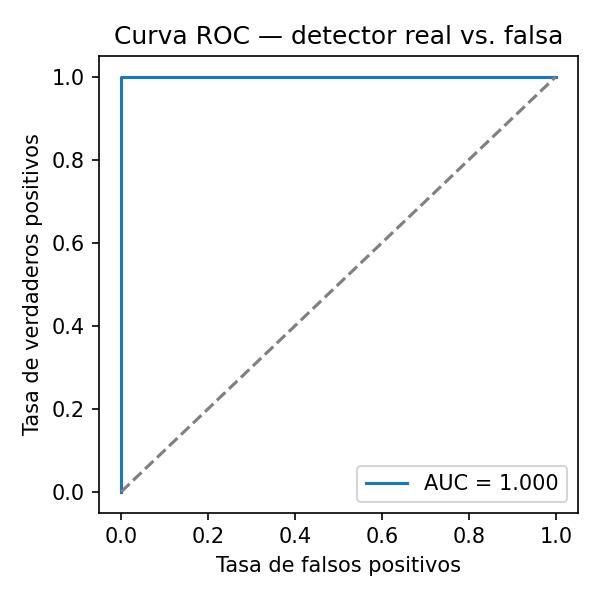
\includegraphics[width=0.8\linewidth]{figures/roc_curve.png}
  \caption{ROC curve of the dual-stream detector on the held-out test set. \pending{regenerar con datos reales}}
  \label{fig:roc}
\end{figure}

\begin{figure}[htbp]
  \centering
  % 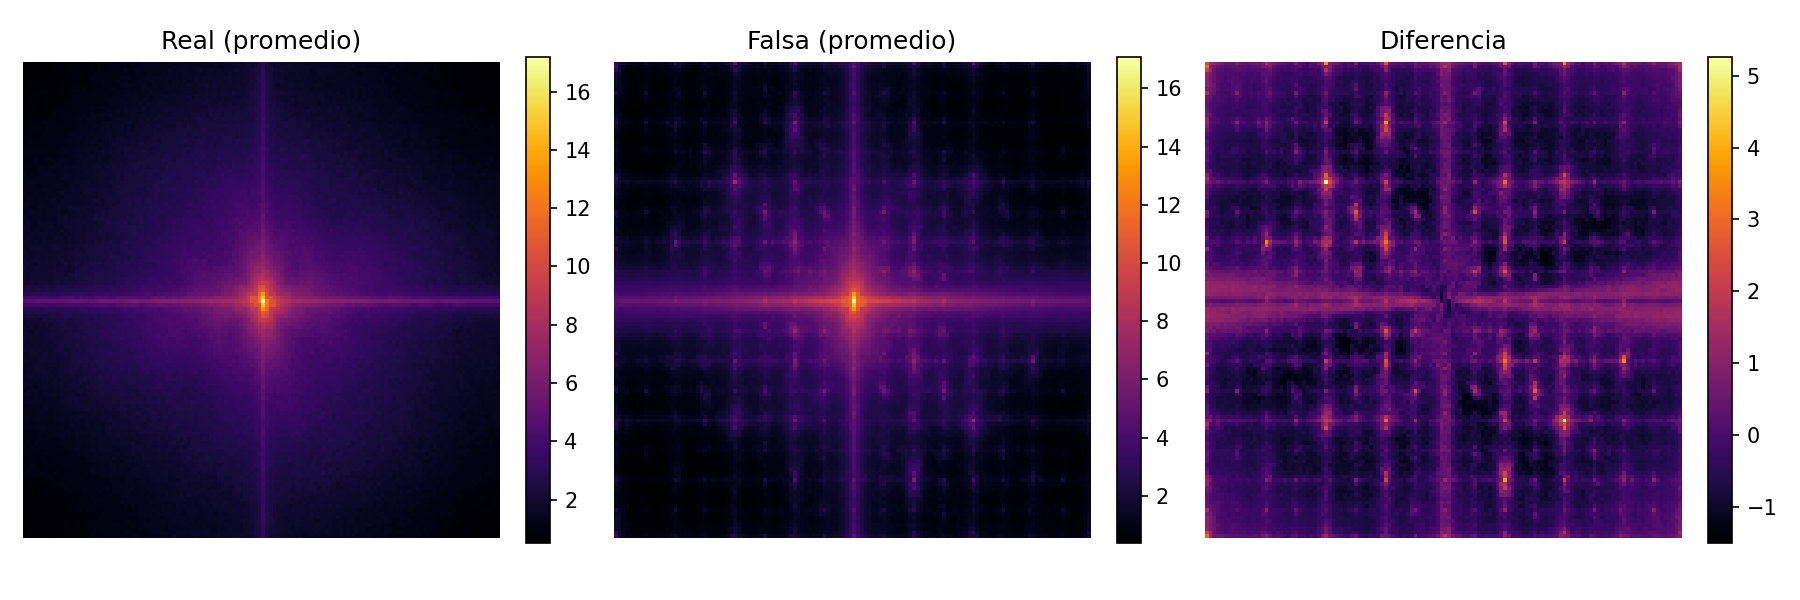
\includegraphics[width=\linewidth]{figures/frequency_spectrum_comparison.png}
  \caption{Average log-power spectrum of real radiographs (left), generated radiographs (center), and their difference (right). The periodic structure visible in the difference map corresponds to the transposed-convolution upsampling artifacts described in Section~\ref{sec:related}. \pending{regenerar con datos reales}}
  \label{fig:freq}
\end{figure}

% -------------------------------------------------------
\section{Discussion and Limitations}
\label{sec:discussion}

\textbf{Dataset scale.} 152 real radiographs is small relative to human-imaging forensics benchmarks such as MedForensics, and results here should be read as a reproducible proof of concept rather than a production-ready fraud detection system. The scarcity itself is evidence for the gap this paper documents: unlike human radiology, veterinary imaging has no equivalent of large public archives (e.g., NIH ChestX-ray14, MIMIC-CXR), because most institutional PACS archives remain closed.

\textbf{GAN vs. diffusion generalization.} Our generator is a DCGAN, not a diffusion model. The human-imaging literature has already shown that detectors trained against GAN artifacts generalize poorly to diffusion-generated images and vice versa \cite{hybrid_gan_diffusion_2026}. Fine-tuning a diffusion model (e.g., via LoRA or DreamBooth) on this same 152-image collection, and testing whether our frequency-domain stream transfers across generator families, is the most direct next step and is left as future work.

\textbf{Scope of imaging modality and species.} The source dataset covers a single view (latero-lateral thoracic) in a single species (canine). Extending this pipeline to feline imaging, abdominal or orthopedic radiographs, and ultrasound would materially increase its relevance to real-world claims review, where fraud is not confined to one view or species.

\textbf{Intended use.} This work is intended as a research contribution and an openly available dataset to seed further study, not as a deployed fraud-detection product. Any operational use in claims adjudication would require substantially larger, prospectively validated data and regulatory/ethical review appropriate to insurance decision-making.

% -------------------------------------------------------
\section{Conclusion}
\label{sec:conclusion}

We identified a real, unaddressed gap between two active but previously disconnected lines of work: the growing literature on detecting AI-generated human medical images, and the well-documented, costly problem of veterinary insurance claims fraud. We built the first publicly available dataset pairing real and AI-generated veterinary radiographs, by legally re-licensing an existing CC BY 4.0 collection and augmenting it with a trained generator, and proposed a dual-stream detector that combines spatial and frequency-domain evidence. We release both the dataset and the full training pipeline to support future work in this niche, including the open question of cross-generator generalization between GANs and diffusion models in veterinary imaging.

% -------------------------------------------------------
\begin{thebibliography}{00}

\bibitem{rsna_deepfake_xray_2026}
Radiological Society of North America, ``Deepfake X-Rays Fool Radiologists and AI,''
RSNA Press Release, \url{https://www.rsna.org/news/2026/march/chatgpt-generated-radiographs}, March 2026.

\bibitem{insurnest_fraud_2026}
Insurnest, ``Pet Insurance Claims Fraud: Common Schemes and How MGAs Detect and Prevent Them,''
\url{https://insurnest.com/blog/pet-insurance-mga-claims-fraud/}, 2026.

\bibitem{medforensics2025}
Authors of MedForensics, ``Toward Medical Deepfake Detection: A Comprehensive Dataset and Novel Method,''
in \textit{Proc. Medical Image Computing and Computer Assisted Intervention (MICCAI)}, 2025.
arXiv:2509.15711.

\bibitem{m3dsynth2023}
G. Pasqualino et al., ``M3Dsynth: A Dataset of Medical 3D Images with AI-Generated Local Manipulations,''
arXiv:2309.07973, 2023.

\bibitem{hybrid_gan_diffusion_2026}
Authors, ``A Hybrid Transfer Learning Approach for Multi-Class Classification of Medical Deepfakes Generated by GAN and Diffusion Models,''
\textit{Discover Computing}, Springer Nature, 2026.

\bibitem{synthetic_review_2026}
Authors, ``A Systematic Review on Synthetic Medical Images Generation: Recent Trends and Future Opportunities,''
\textit{Diagnostics}, vol. 16, no. 14, 2026.

\bibitem{frequency_checkerboard_2021}
Y. Nataraj et al. (representative work), ``A Universal Detector of CNN-Generated Images Using Properties of Checkerboard Artifacts in the Frequency Domain,''
arXiv:2108.01892, 2021.

\bibitem{vet_quality_2024}
S. Tahghighi et al., ``Classification of the Quality of Canine and Feline Ventrodorsal and Dorsoventral Thoracic Radiographs through Machine Learning,''
\textit{Veterinary Radiology \& Ultrasound}, 2024.

\bibitem{vet_symmetry_2023}
Authors, ``Automatic Classification of Symmetry of Hemithoraces in Canine and Feline Radiographs,''
arXiv:2302.12923, 2023.

\bibitem{mendeley_vhs_dataset}
C. A. Flores Dueñas, S. M. Gaxiola Camacho, and M. F. Montaño Gómez,
``Radiographic Dataset for VHS Determination Learning Process,''
\textit{Mendeley Data}, V1, doi: 10.17632/ktx4cj55pn.1, 2022.

\bibitem{dcgan_radford2015}
A. Radford, L. Metz, and S. Chintala,
``Unsupervised Representation Learning with Deep Convolutional Generative Adversarial Networks,''
arXiv:1511.06434, 2015.

\end{thebibliography}

\end{document}
